\begin{frame}{Image Classification}
\begin{itemize}
    \item We can represent an image as a vector in a very high dimensional space, $\mathbb{R}^D$
    \begin{figure}
    \centering
    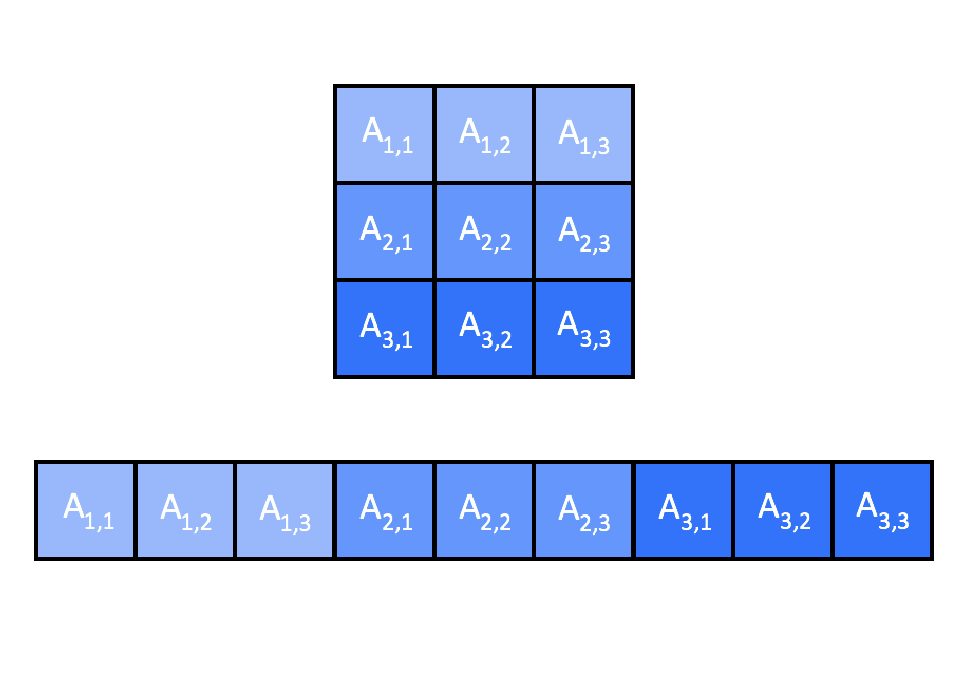
\includegraphics[width=0.6\textwidth]{img/flatten.png}
    
    \caption{Flatten a matrix $A$ into a vector\footnote{quantstart.com}}
    \end{figure}
\end{itemize}

\end{frame}

\begin{frame}{Image Classification}
\begin{itemize}
    \item After flattening image $\textbf{x} \in \mathbb{R}^D$, we want to classify as cat/ not cat using logistic regression
    $$y = \sigma(w_0 + w_1x_1 + ... + w_Dx_D)$$
    where each $x_i \in \textbf{x}$ is a value for one pixel in one RGB channel.
    \begin{figure}
    \centering
    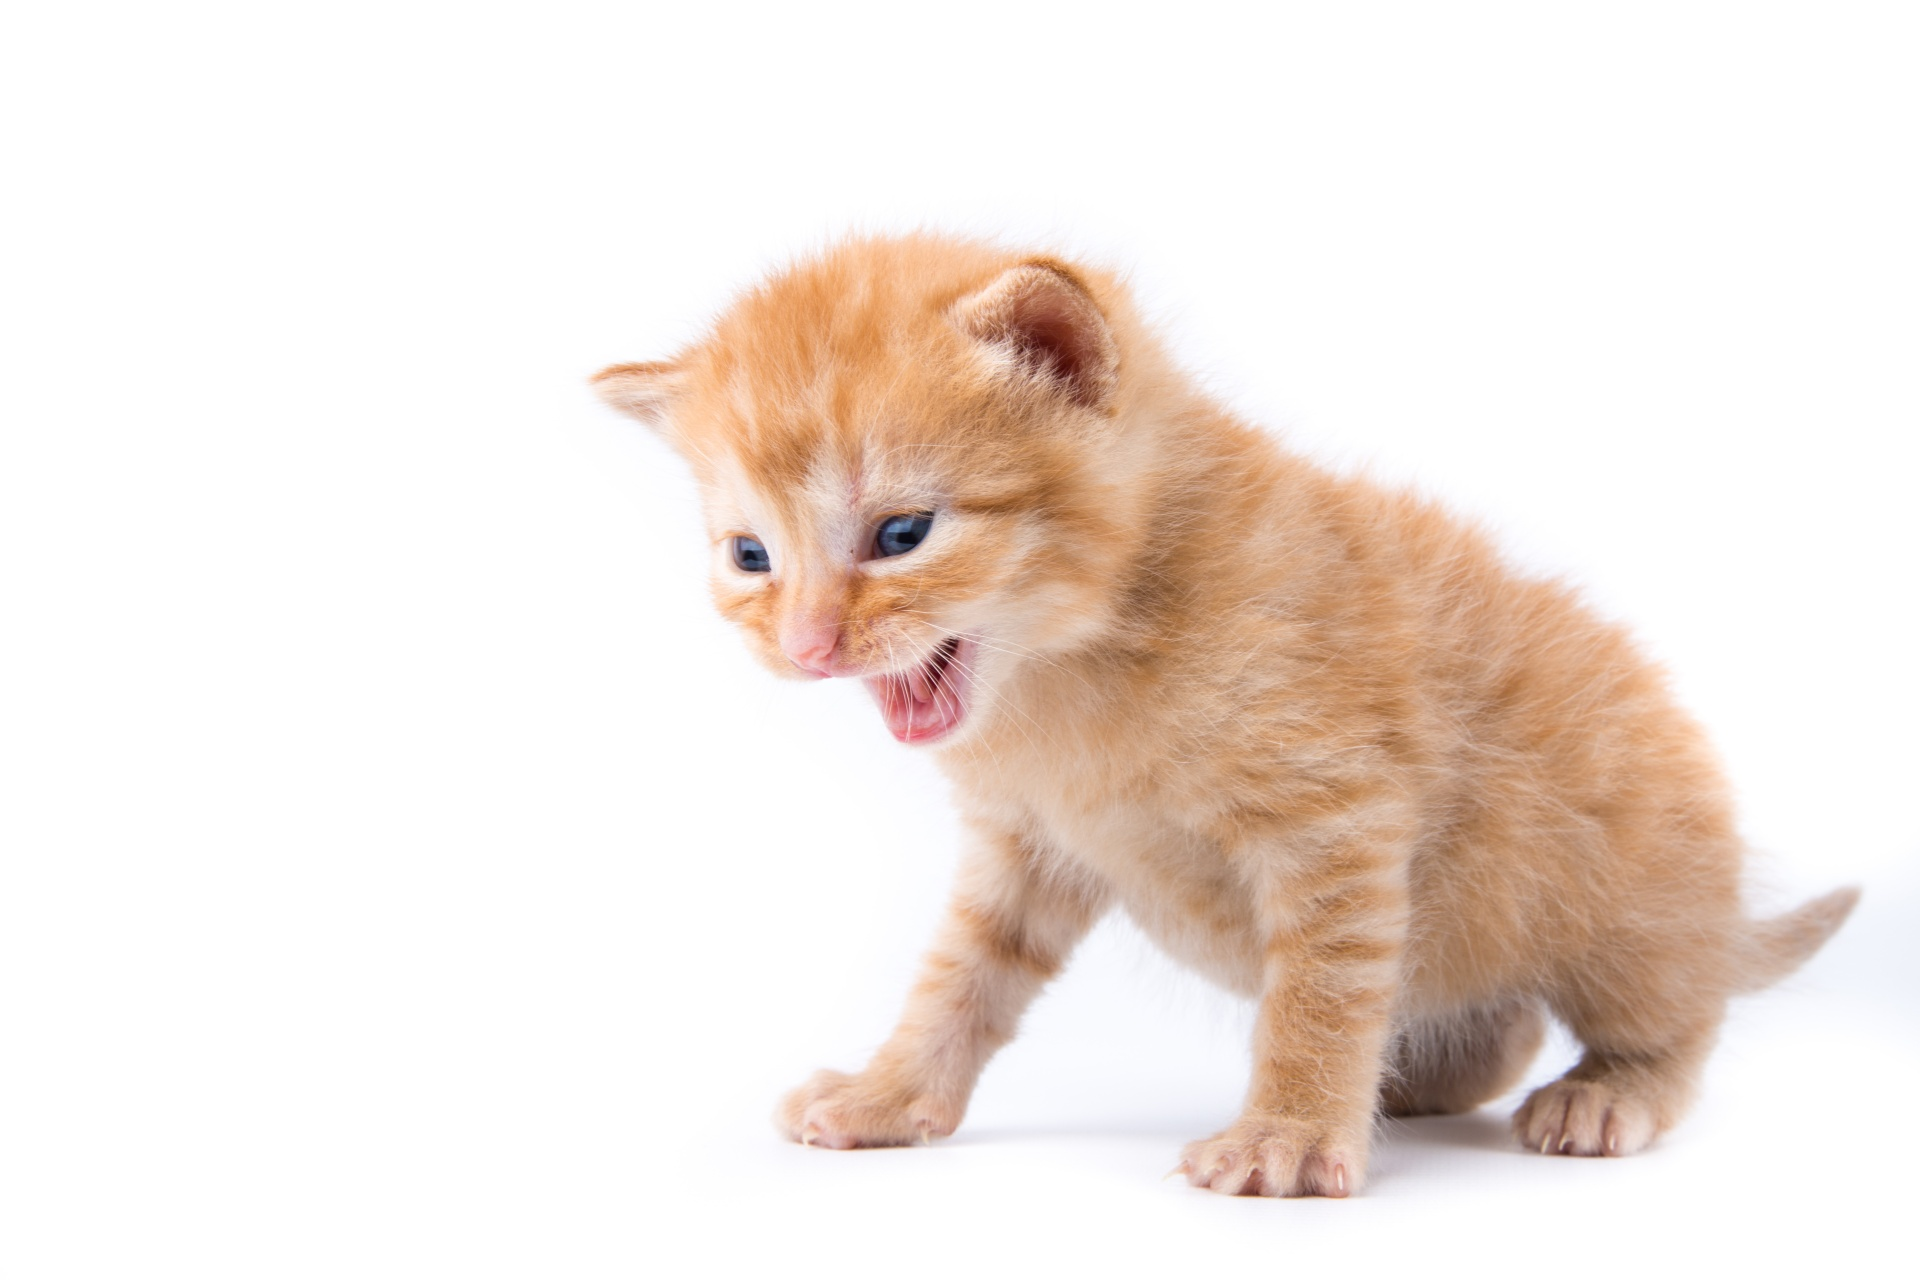
\includegraphics[width=0.6\textwidth]{img/cat.jpg}
    \end{figure}
    \item What could be a problem with this approach?
\end{itemize}
\end{frame}

\begin{frame}{Image Classification}
\begin{itemize}
    \item Interpretation of linear classifiers as template matching. 
    \item Weights W corresponds to a template for the cat class. 
    \item Whether or not an image is a cat is decided by comparing the template with the image using dot product to find if the score exceeds the $0.5$ decision boundary.
\end{itemize}
\end{frame}

\begin{frame}{Image Classification}
    \begin{figure}
    \centering
    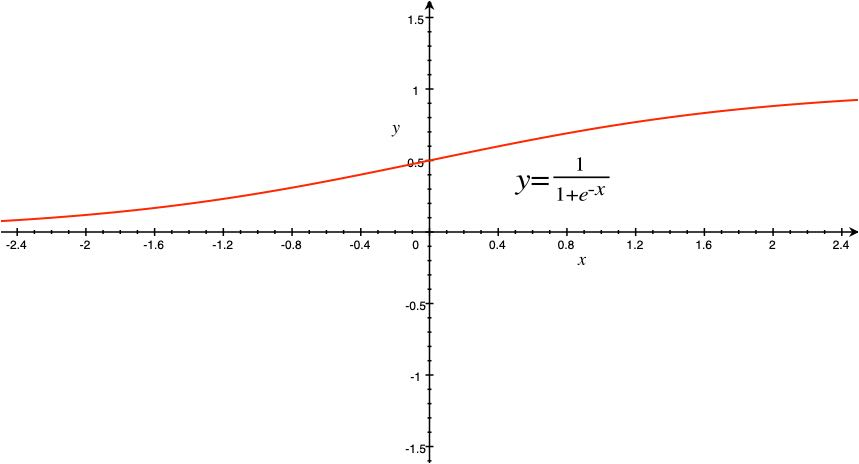
\includegraphics[width=0.8\textwidth]{img/sigmoid.jpg}
    \caption{The sigmoid function $\sigma$ will predict cat for higher value of $\textbf{x} \cdot \textbf{w}$, and not cat for lower.}
    \end{figure}
\end{frame}

\begin{frame}{Image Classification}
\begin{itemize}
    \item Interpretation of linear classifiers as template matching. 
    \item Weights W corresponds to a template for the cat class. 
    \item Whether or not an image is a cat is decided by comparing the template with the image using dot product to find if the score exceeds the $0.5$ decision boundary.
    \item \textbf{The best template should look approximately like a cat!}
\end{itemize}
\end{frame}

\begin{frame}{Image Classification}
    \begin{figure}
    \centering
    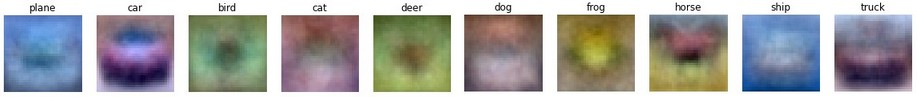
\includegraphics[width=\textwidth]{img/templates.jpg}
    \caption{Using gradient descent, the weights $\textbf{w}$ learn a visual resemblance of a class}
    \end{figure}
    \begin{itemize}
        \item Now, what do you think you this is a problem with these templates?
    \end{itemize}
     \footnotetext{cs231n.github.io/linear-classify}
\end{frame}

\begin{frame}{Image Classification}
    \begin{figure}
    \centering
    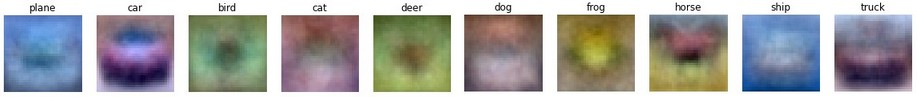
\includegraphics[width=\textwidth]{img/templates.jpg}
    \caption{Using gradient descent, the weights $\textbf{w}$ learn a visual resemblance of a class}
    \end{figure}
    \begin{itemize}
        \item Now, what do you think you this is a problem with these templates?
        \item It is very hard to capture all possible variations of an image using just a single template.
    \end{itemize}
     \footnotetext{cs231n.github.io/linear-classify}
\end{frame}